 \documentclass[conference]{IEEEtran}
\usepackage{blindtext, graphicx}
\usepackage{amssymb,amsmath}
\usepackage{siunitx}

\usepackage{multicol}
\usepackage[linesnumbered,ruled]{algorithm2e}
\usepackage[noend]{algpseudocode}
\usepackage{mdframed,framed}

\usepackage{tikz}
\newcommand*\circled[1]{\tikz[baseline=(char.base)]{
            \node[shape=circle,draw,inner sep=0.3pt] (char) {#1};}}
\usetikzlibrary{positioning,chains,fit,shapes,calc}
% Some very useful LaTeX packages include:
% (uncomment the ones you want to load)
%----------------------------------------------------------------------------------------
%	LISTINGS
%----------------------------------------------------------------------------------------
\usepackage{verbatim}
\usepackage{xcolor}
\definecolor{bgcolor}{rgb}{0.98,0.98,0.98}
\definecolor{light-gray}{gray}{0.95}
\usepackage{listings}
\lstset{language=C}
\lstset{
  basicstyle=\footnotesize\ttfamily,
  breaklines=true,
  showstringspaces=false,
  numbers=none,
  backgroundcolor=\color{white},
  commentstyle=\color{red},
  keywordstyle=\color{black}\bfseries,
  keywordstyle=[1]\color{black},   % cyan or teal can also be a good choice, use \bfseries for bold
  frame=none,                     % adds a frame around the code
  %xleftmargin=\parindent,
  tabsize=2,                      % sets default tabsize to 2 spaces
  captionpos=b,                   % sets the caption-position to bottom
  morekeywords=[1]{               % if you want to add more keywords to the set
    MODELTYPE,
    __CALCL_MODEL_3D,
    MODEL_2D,
    MODEL_3D,
    CALCLcontext,
    CALCLdevice,
    CALCLkernel,
    CALCLManager,
    CALCLmem,
    CALCLModel2D,
    CALCLModel3D,
    CALCLprogram,
    CAL_CUSTOM_NEIGHBORHOOD_2D,
    CAL_CUSTOM_NEIGHBORHOOD_3D,
    CAL_FALSE,
    CALGL_DATA_TYPE_DYNAMIC,
    CALGL_DRAW_MODE_FLAT,
    CALGL_DRAW_MODE_SURFACE,
    CALGL_INFO_BAR_ORIENTATION_VERTICAL,
    CALGL_TYPE_INFO_USE_CURRENT_COLOR,
    CALGL_TYPE_INFO_USE_RED_YELLOW_SCALE,
    CALGL_TYPE_INFO_USE_NO_COLOR,
    CALGL_TYPE_INFO_COLOR_DATA,
    CALGL_TYPE_INFO_NORMAL_DATA,
    CALGL_TYPE_INFO_VERTEX_DATA,
    CALGL_TYPE_INFO_USE_CONST_VALUE,
    CALGL_TYPE_INFO_USE_DEFAULT,
    CALGL_TYPE_INFO_USE_RED_SCALE,
    CALGL_DATA_TYPE_STATIC,
    CALGLRun2D,
    CALGLRun3D,
    CALGLDrawModel2D,
    CALGLDrawModel3D,
    CAL_HEXAGONAL_NEIGHBORHOOD_2D,
    CAL_HEXAGONAL_NEIGHBORHOOD_ALT_2D,
    CAL_MOORE_NEIGHBORHOOD_2D,
    CAL_MOORE_NEIGHBORHOOD_3D,
    CAL_NO_OPT,
    CAL_OPT_ACTIVE_CELLS,
    CAL_RUN_LOOP,
    CAL_SPACE_FLAT,
    CAL_SPACE_TOROIDAL,
    CAL_TRUE,
    CAL_UPDATE_EXPLICIT,
    CAL_UPDATE_IMPLICIT,
    CAL_VON_NEUMANN_NEIGHBORHOOD_2D,
    CAL_VON_NEUMANN_NEIGHBORHOOD_3D,
    calAddActiveCell2D,
    calAddActiveCell3D,
    calAddActiveCellX2D,
    calAddActiveCellX3D,
    calAddElementaryProcess2D,
    calAddElementaryProcess3D,
    calAddSingleLayerSubstate2Db,
    calAddSingleLayerSubstate2Di,
    calAddSingleLayerSubstate2Dr,
    calAddSingleLayerSubstate3Db,
    calAddSingleLayerSubstate3Di,
    calAddSingleLayerSubstate3Dr,
    calAddSubstate2Db,
    calAddSubstate2Di,
    calAddSubstate2Dr,
    calAddSubstate3Db,
    calAddSubstate3Di,
    calAddSubstate3Dr,
    calAddActiveCell2D,
    calAddActiveCellX2D,
    calAddActiveCell3D,
    calAddActiveCellX3D,
    calApplyElementaryProcess2D,
    calApplyElementaryProcess3D,
    CALbyte,
    calclAddActiveCell2D,
    calclAddActiveCellX2D,
    calclAddElementaryProcess2D,
    calclAddElementaryProcess3D,
    calclAddReductionSum2Di,
    calclAddStopConditionFunc2D,
    calclAddStopConditionFunc3D,
    calclAddSteeringFunc2D,
    calclAddSteeringFunc3D,
    calclCreateBuffer,
    calclCreateContext,
    calclCreateManager,
    calCADef2D,
    calCADef3D,
    calclCADef2D,
    calclCADef3D,
    calclFinalizeManager,
    calclFinalize2D,
    calclFinalize3D,
    calclGet2Db,
    calclGet3Db,
    calclGet2Di,
    calclGet3Di,
    calclGet2Dr,
    calclGet3Dr,
    calclGetX2Db,
    calclGetX2Di,
    calclGetX2Dr,
    calclGetX3Db,
    calclGetX3Di,
    calclGetX3Dr,
    calclGetDevice,
    calclGetSum2Di,
    calclGlobalRow,
    calclGlobalColumn,
    calclGlobalSlice,
    calclInitializePlatforms,
    calclInitializeDevices,
    calclLoadProgram2D,
    calclLoadProgram3D,
    calclLocalRow,
    calclLocalColumn,
    calclLocalSlice,
    calclGetKernelFromProgram,
    calclGetRows,
    calclGetColumns,
    calclGetSlices,
    calclgGetByteSubstatesNum,
    calclGetIntSubstatesNum,
    calclGetRealSubstatesNum,
    calclGetCurrentByteSubstates,
    calclGetCurrentIntSubstates,
    calclGetCurrentRealSubstates,
    calclGetNextByteSubstates,
    calclGetNextIntSubstates,
    calclGetNnextRealSubstates,
    calclGetNeighborhood,
    calclGetNeighborhoodID,
    calclGetNeighborhoodSize,
    calclGetBoundaryCondition,
    calclGetPlatformAndDeviceFromStdIn,
    calclRemoveActiveCell2D,
    calclRemoveActiveCell3D,
    calclRun2D,
    calclRun3D,
    calclRunStop,
    calclSetKernelArg2D,
    calclSetKernelArg3D,
    calclThreadCheck2D,
    calclThreadCheck2D,
    calclSet2Db,
    calclSet3Db,
    calclSet2Di,
    calclSet3Di,
    calclSet2Dr,
    calclSet3Dr,
    calclActiveThreadCheck2D,
    calclActiveThreadCheck3D,
    CALDrawModel2D,
    CALDrawModel3D,
    calFinalize2D,
    calFinalize3D,
    calGet2Db,
    calGet2Di,
    calGet2Dr,
    calGet3Db,
    calGet3Di,
    calGet3Dr,
    calGetX2Db,
    calGetX2Di,
    calGetX2Dr,
    calGetX3Db,
    calGetX3Di,
    calGetX3Dr,
    calglAdd2Db,
    calglAdd3Db,
    calglAdd2Di,
    calglAdd3Di,
    calglAdd2Dr,
    calglAdd3Dr,
    calglColor2D,
    calglColor3D,
    calglDefDrawModel2D,
    calglDefDrawModel3D,
    calglDefDrawModelCL2D,
    calglDefDrawModelCL3D,
    calglDisplayDrawJBound2D,
    calglHideDrawJBound2D,
    calglInfoBar2Dr,
    calglInitViewer,
    calglMainLoop2D,
    calglMainLoop3D,
    calglRelativeInfoBar2Dr,
    calglRelativeInfoBar3Dr,
    calglRunCLDef2D,
    calglRunCLDef3D,
    calglSetDisplayStep,
    calglSetHeightOffset2D,
    calglSetHeightOffset3D,
    calInit2Db,
    calInit2Di,
    calInit2Dr,
    calInit3Db,
    calInit3Di,
    calInit3Dr,
    calInitSubstate2Db,
    calInitSubstate2Di,
    calInitSubstate2Dr,
    calInitSubstate3Db,
    calInitSubstate3Di,
    calInitSubstate3Dr,
    CALint,
    calLoadSubstate2Db,
    calLoadSubstate2Di,
    calLoadSubstate2Dr,
    calLoadSubstate3Db,
    calLoadSubstate3Di,
    calLoadSubstate3Dr,
    CALModel2D,
    CALModel3D,
    CALNeighborhood2D,
    CALNeighborhood3D,
    CALOptimization,
    CALParameterb,
    CALParameteri,
    CALParameterr,
    CALreal,
    calRemoveActiveCell2D,
    calRemoveActiveCell3D,
    CALRun2D,
    CALRun3D,
    calRun2D,
    calRun3D,
    calRunAddGlobalTransitionFunc2D,
    calRunAddGlobalTransitionFunc3D,
    calRunAddInitFunc2D,
    calRunAddInitFunc3D,
    calRunAddSteeringFunc2D,
    calRunAddSteeringFunc3D,
    calRunAddStopConditionFunc2D,
    calRunAddStopConditionFunc3D,
    calRunDef2D,
    calRunDef3D,
    calRunInitSimulation2D,
    calRunInitSimulation3D,
    calRunFinalize2D,
    calRunFinalize3D,
    calRunFinalizeSimulation2D,
    calRunFinalizeSimulation3D,
    calSaveSubstate2Db,
    calSaveSubstate2Di,
    calSaveSubstate2Dr,
    calSaveSubstate3Db,
    calSaveSubstate3Di,
    calSaveSubstate3Dr,
    calSet2Db,
    calSet2Di,
    calSet2Dr,
    calSet3Db,
    calSet3Di,
    calSet3Dr,
    calSetX2Db,
    calSetX2Di,
    calSetX2Dr,
    calSetX3Db,
    calSetX3Di,
    calSetX3Dr,
    calSetCurrent2Db,
    calSetCurrent2Di,
    calSetCurrent2Dr,
    calSetCurrent3Db,
    calSetCurrent3Di,
    calSetCurrent3Dr,
    CALSpaceBoundaryCondition,
    CALSubstate2Db,
    CALSubstate2Di,
    CALSubstate2Dr,
    CALSubstate3Db,
    CALSubstate3Di,
    CALSubstate3Dr,
    calUpdateActiveCells2D,
    calUpdateSubstate2Db,
    calUpdateSubstate2Di,
    calUpdateSubstate2Dr,
    calUpdate2D,
    calUpdate3D,
    CALUpdateMode,
    }
}




%----------------------------------------------------------------------------------------
%	ALGORITHM
%----------------------------------------------------------------------------------------
%\usepackage[]{algorithm2e}



%\SetKwProg{Fn}{Procedure}{}{}


% *** MISC UTILITY PACKAGES ***
%
%\usepackage{ifpdf}
% Heiko Oberdiek's ifpdf.sty is very useful if you need conditional
% compilation based on whether the output is pdf or dvi.
% usage:
% \ifpdf
%   % pdf code
% \else
%   % dvi code
% \fi
% The latest version of ifpdf.sty can be obtained from:
% http://www.ctan.org/tex-archive/macros/latex/contrib/oberdiek/
% Also, note that IEEEtran.cls V1.7 and later provides a builtin
% \ifCLASSINFOpdf conditional that works the same way.
% When switching from latex to pdflatex and vice-versa, the compiler may
% have to be run twice to clear warning/error messages.







%\usepackage{cite}






% *** MATH PACKAGES ***
%
%\usepackage[cmex10]{amsmath}
% A popular package from the American Mathematical Society that provides
% many useful and powerful commands for dealing with mathematics. If using
% it, be sure to load this package with the cmex10 option to ensure that
% only type 1 fonts will utilized at all point sizes. Without this option,
% it is possible that some math symbols, particularly those within
% footnotes, will be rendered in bitmap form which will result in a
% document that can not be IEEE Xplore compliant!
%
% Also, note that the amsmath package sets \interdisplaylinepenalty to 10000
% thus preventing page breaks from occurring within multiline equations. Use:
%\interdisplaylinepenalty=2500
% after loading amsmath to restore such page breaks as IEEEtran.cls normally
% does. amsmath.sty is already installed on most LaTeX systems. The latest
% version and documentation can be obtained at:
% http://www.ctan.org/tex-archive/macros/latex/required/amslatex/math/





% *** SPECIALIZED LIST PACKAGES ***
%

% algorithmic.sty was written by Peter Williams and Rogerio Brito.
% This package provides an algorithmic environment fo describing algorithms.
% You can use the algorithmic environment in-text or within a figure
% environment to provide for a floating algorithm. Do NOT use the algorithm
% floating environment provided by algorithm.sty (by the same authors) or
% algorithm2e.sty (by Christophe Fiorio) as IEEE does not use dedicated
% algorithm float types and packages that provide these will not provide
% correct IEEE style captions. The latest version and documentation of
% algorithmic.sty can be obtained at:
% http://www.ctan.org/tex-archive/macros/latex/contrib/algorithms/
% There is also a support site at:
% http://algorithms.berlios.de/index.html
% Also of interest may be the (relatively newer and more customizable)
% algorithmicx.sty package by Szasz Janos:
% http://www.ctan.org/tex-archive/macros/latex/contrib/algorithmicx/




% *** ALIGNMENT PACKAGES ***
%
%\usepackage{array}
% Frank Mittelbach's and David Carlisle's array.sty patches and improves
% the standard LaTeX2e array and tabular environments to provide better
% appearance and additional user controls. As the default LaTeX2e table
% generation code is lacking to the point of almost being broken with
% respect to the quality of the end results, all users are strongly
% advised to use an enhanced (at the very least that provided by array.sty)
% set of table tools. array.sty is already installed on most systems. The
% latest version and documentation can be obtained at:
% http://www.ctan.org/tex-archive/macros/latex/required/tools/


%\usepackage{mdwmath}
%\usepackage{mdwtab}
% Also highly recommended is Mark Wooding's extremely powerful MDW tools,
% especially mdwmath.sty and mdwtab.sty which are used to format equations
% and tables, respectively. The MDWtools set is already installed on most
% LaTeX systems. The lastest version and documentation is available at:
% http://www.ctan.org/tex-archive/macros/latex/contrib/mdwtools/


% IEEEtran contains the IEEEeqnarray family of commands that can be used to
% generate multiline equations as well as matrices, tables, etc., of high
% quality.


%\usepackage{eqparbox}
% Also of notable interest is Scott Pakin's eqparbox package for creating
% (automatically sized) equal width boxes - aka "natural width parboxes".
% Available at:
% http://www.ctan.org/tex-archive/macros/latex/contrib/eqparbox/





% *** SUBFIGURE PACKAGES ***
%\usepackage[tight,footnotesize]{subfigure}
% subfigure.sty was written by Steven Douglas Cochran. This package makes it
% easy to put subfigures in your figures. e.g., "Figure 1a and 1b". For IEEE
% work, it is a good idea to load it with the tight package option to reduce
% the amount of white space around the subfigures. subfigure.sty is already
% installed on most LaTeX systems. The latest version and documentation can
% be obtained at:
% http://www.ctan.org/tex-archive/obsolete/macros/latex/contrib/subfigure/
% subfigure.sty has been superceeded by subfig.sty.



%\usepackage[caption=false]{caption}
%\usepackage[font=footnotesize]{subfig}
% subfig.sty, also written by Steven Douglas Cochran, is the modern
% replacement for subfigure.sty. However, subfig.sty requires and
% automatically loads Axel Sommerfeldt's caption.sty which will override
% IEEEtran.cls handling of captions and this will result in nonIEEE style
% figure/table captions. To prevent this problem, be sure and preload
% caption.sty with its "caption=false" package option. This is will preserve
% IEEEtran.cls handing of captions. Version 1.3 (2005/06/28) and later 
% (recommended due to many improvements over 1.2) of subfig.sty supports
% the caption=false option directly:
%\usepackage[caption=false,font=footnotesize]{subfig}
%
% The latest version and documentation can be obtained at:
% http://www.ctan.org/tex-archive/macros/latex/contrib/subfig/
% The latest version and documentation of caption.sty can be obtained at:
% http://www.ctan.org/tex-archive/macros/latex/contrib/caption/




% *** FLOAT PACKAGES ***
%
%\usepackage{fixltx2e}
% fixltx2e, the successor to the earlier fix2col.sty, was written by
% Frank Mittelbach and David Carlisle. This package corrects a few problems
% in the LaTeX2e kernel, the most notable of which is that in current
% LaTeX2e releases, the ordering of single and double column floats is not
% guaranteed to be preserved. Thus, an unpatched LaTeX2e can allow a
% single column figure to be placed prior to an earlier double column
% figure. The latest version and documentation can be found at:
% http://www.ctan.org/tex-archive/macros/latex/base/



%\usepackage{stfloats}
% stfloats.sty was written by Sigitas Tolusis. This package gives LaTeX2e
% the ability to do double column floats at the bottom of the page as well
% as the top. (e.g., "\begin{figure*}[!b]" is not normally possible in
% LaTeX2e). It also provides a command:
%\fnbelowfloat
% to enable the placement of footnotes below bottom floats (the standard
% LaTeX2e kernel puts them above bottom floats). This is an invasive package
% which rewrites many portions of the LaTeX2e float routines. It may not work
% with other packages that modify the LaTeX2e float routines. The latest
% version and documentation can be obtained at:
% http://www.ctan.org/tex-archive/macros/latex/contrib/sttools/
% Documentation is contained in the stfloats.sty comments as well as in the
% presfull.pdf file. Do not use the stfloats baselinefloat ability as IEEE
% does not allow \baselineskip to stretch. Authors submitting work to the
% IEEE should note that IEEE rarely uses double column equations and
% that authors should try to avoid such use. Do not be tempted to use the
% cuted.sty or midfloat.sty packages (also by Sigitas Tolusis) as IEEE does
% not format its papers in such ways.





% *** PDF, URL AND HYPERLINK PACKAGES ***
%
\usepackage{url}
% url.sty was written by Donald Arseneau. It provides better support for
% handling and breaking URLs. url.sty is already installed on most LaTeX
% systems. The latest version can be obtained at:
% http://www.ctan.org/tex-archive/macros/latex/contrib/misc/
% Read the url.sty source comments for usage information. Basically,
% \url{my_url_here}.





% *** Do not adjust lengths that control margins, column widths, etc. ***
% *** Do not use packages that alter fonts (such as pslatex).         ***
% There should be no need to do such things with IEEEtran.cls V1.6 and later.
% (Unless specifically asked to do so by the journal or conference you plan
% to submit to, of course. )


% correct bad hyphenation here
\hyphenation{op-tical net-works semi-conduc-tor}

\usepackage{lipsum}
\begin{document}
%
% paper title
% can use linebreaks \\ within to get better formatting as desired
\title{TraCCA -  A Complex Cellular Automata based Particle Tracking Framework }


% author names and affiliations
% use a multiple column layout for up to three different
% affiliations
\author{\IEEEauthorblockN{Davide Spataro, Paola Arcuri, Alessio De Rango,\\ William Spataro
    and Donato D'Ambrosio}
\IEEEauthorblockA{Department of Mathematics and Computer Science\\
University of Calabria\\
Rende, Italy\\
Email: d.spataro@mat.unical.it}
\and
\IEEEauthorblockN{ Alice Mari}
\IEEEauthorblockA{Institute for BioEngineering\\
University of Edinburgh\\
King’s Buildings, EH9 3BF Edinburgh, UK\\
Email: alicemari45@gmail.com }
}
% conference papers do not typically use \thanks and this command
% is locked out in conference mode. If really needed, such as for
% the acknowledgment of grants, issue a \IEEEoverridecommandlockouts
% after \documentclass

% for over three affiliations, or if they all won't fit within the width
% of the page, use this alternative format:
% 
%\author{\IEEEauthorblockN{Michael Shell\IEEEauthorrefmark{1},
%Homer Simpson\IEEEauthorrefmark{2},
%James Kirk\IEEEauthorrefmark{3}, 
%Montgomery Scott\IEEEauthorrefmark{3} and
%Eldon Tyrell\IEEEauthorrefmark{4}}
%\IEEEauthorblockA{\IEEEauthorrefmark{1}School of Electrical and Computer Engineering\\
%Georgia Institute of Technology,
%Atlanta, Georgia 30332--0250\\ Email: see http://www.michaelshell.org/contact.html}
%\IEEEauthorblockA{\IEEEauthorrefmark{2}Twentieth Century Fox, Springfield, USA\\
%Email: homer@thesimpsons.com}
%\IEEEauthorblockA{\IEEEauthorrefmark{3}Starfleet Academy, San Francisco, California 96678-2391\\
%Telephone: (800) 555--1212, Fax: (888) 555--1212}
%\IEEEauthorblockA{\IEEEauthorrefmark{4}Tyrell Inc., 123 Replicant Street, Los Angeles, California 90210--4321}}




% use for special paper notices
%\IEEEspecialpapernotice{(Invited Paper)}




% make the title area
\maketitle


\begin{abstract}
%\lipsum[1-1]
Particle tracking plays an important role in numerous fields of science for the investigation of the movement of sub-micron particles, micropsheres and molecules under microscopic observation.
In this paper we present an algorithm for detecting and tracking particles based on geometrical difference evaluation and centroid displacement analysis to reconstruct the trajectories. 
This method works for $n$-dimensional input data provided that particles are represented by at least a centroid space coordinate and a geometrical entity which describe their shape. 
Since 2-D images are a common source of such data, we also present a framework for image-manipulation based on Extended Cellular Automata (XCA).
We have applied and validated TraCCA in investigating the motility of \textit{B. subtilis.} injected in a microfluidic device using 4100 images taken at 100 frames per second. 
Results show that the framework is able to reconstruct the trajectories as computed motion parameters that are in accordance with the ones found in literature. Eventually, a preliminary parallel version implemented on GPUs and distributed memory machines have produced promising scalability and speedup, proving that the methodology can be also applied for large datasets.  


\end{abstract}

% Note that keywords are not normally used for peerreview papers.
\begin{IEEEkeywords}
cellular automata, tracking, image processing, bacteria motility
\end{IEEEkeywords}






% For peer review papers, you can put extra information on the cover
% page as needed:
% \ifCLASSOPTIONpeerreview
% \begin{center} \bfseries EDICS Category: 3-BBND \end{center}
% \fi
%
% For peerreview papers, this IEEEtran command inserts a page break and
% creates the second title. It will be ignored for other modes.
\IEEEpeerreviewmaketitle

\section{Introduction}
Studying of the movement of sub-micron particles, micro-spheres and molecules under microscopic observation often requires their time trajectories from which important kinematic and dynamic properties can be computed. 
Several studies employ time-lapse microscopy, especially in the field of biophysics, as a tool to gather data and retrieve single particle time trajectories. The researcher usually relies on manual or semi-manual/interactive software to study such properties. However, this approach is unfeasible when the number of cells involved in the analysis is high.

In this paper we present an algorithm for detecting and tracking particles that is based on image processing techniques and to shape difference and centroid displacement analysis to reconstruct the trajectories. 
This method works for $n$-dimensional input data provided that particles are represented by at least a centroid space coordinate and a geometrical entity which describe its shape. 
Since $2$D images are a common source of such data we also present framework for image-manipulation based on the Extended Cellular Automata(XCA) paradigm .

TraCCA has been successfully applied for the investigation of the motility of \textit{B. subtilis.} injected in a micro-fluidic device using 4100 images taken at 100 frames per second, as reported in Section \ref{sect:bacteriaanalysis}.

The paper is organized as follows: Sections  \ref{trackalgorithm} and \ref{manipulating} outline the proposed tracking algorithm and cellular automata based image processing framework, respectively; Section \ref{sect:bacteriaanalysis} shows a detailed application of TraCCA referred to a real case study regarding bacterial motility, while conclusions and possible future works are reported in Section \ref{conclusions}.



\section{Tracking Algorithm}\label{trackalgorithm}
The objective of the tracking algorithm is to produce a 
set $ T_n = \{ t_i \}$  s.t.  $t_i=\{ c^i_k,c^i_{k+1},\ldots,c^i_l \} $ 
of trajectories each described as a time-ordered list of positions in space from a set of input 
particles $P=P_1 \cup P_2 \cup \ldots \cup P_n$ and a function $\mathcal{D} :  P \times P \mapsto \mathbb{R}$, 
the \textit{distance} function. $P_i = \{p^j_i \; | \; 1 \leq j\; \}$ indicates all particles at time $i$ and each particle $p_i^j$ is defined by a centroid position, and a bounding box which describes its geometrical properties.
$\mathcal{D}(p,q)$ measures the likeliness that a particle $p$ has been transformed into $q$ as a result of the application of a number of geometrical transformations such as translation, scaling, shearing or rotation (see Eq. \ref{sec:bacttracking}). 
Indexes $k$ and $l$, $k \leq l$ indicate the trajectory starting and ending time of the tracked movement respectively, and the length $l-k+1$ is its duration in time.
Note that particles may appear or disappear at any time and hence $k\geq 0$ and $l \leq n$. Moreover, $|t_i| \leq l-k+1$ since a particle which has been successfully tracked
 from  $P_k$ to $P_{k^*} $ can disappear for a certain time and may appear again in $P_{\bar{k}}$, $k \leq k^* \leq \bar{k}$. We only allow disappearing time $\bar{k}-k^* \leq \xi$ where $\xi \geq 0$ is a parameter of the algorithm. 
Each trajectory  $t_*=\{ c^*_k,c^*_{k+1},\ldots,c^*_l \} $ is composed by  positions of particles $p^{j_1}_k,p^{j_2}_{k+1},\ldots,p^{j_*}_l$ at different times. 
This means that, for our purpose, particle $p^{j_1}_k$ at frame $k$ has moved from $c^*_k$ to location of particle $p^{j_2}_{k+1}$,$c^*_{k+1}$ at time ${k+1}$ and to location of $p^{j_*}_{l}$, $c^*_l$ at time $l$. 

As an example, let us consider a human tracking system where each $P_i$ could correspond to all the detected bodies in a  video frame $i$ and the distance function a linear combination of the euclidean distance between two detected bodies centroids  and pixel-by-pixel difference in colors of all the pixels within their bounding boxes. In this context, it would make sense to consider a not null disappearing time since it is not uncommon for the human detection module (which is in charge of producing the centroids and bounding box from the images) to skip recognizing a specific target only for a limited number of frames. 


In order to construct the trajectories, the algorithm works sequentially from frame $1$ to $n$ processing, at each step, two subsets of particles, $M_i$ and $P_{i}$, where $M_i$ contains all the corresponding trajectories ending particles $p^{j}_l$ that can still be expanded, i.e. $i-l \leq \xi$ .
Informally, the algorithm tries to augment an element in $M_i$ using a particle in $P_i$ making sure at most one particle is added to it, the same particle does not augment two different trajectories and the augmenting is performed s.t. the distance function is minimized.

Since at each step of the process a possible assignment between an element of $M_i$ and one of $P_i$ is sought, the algorithm can be thought to be similar to the \textit{assignment problem} \cite{bellmann1978} and more specifically, it consists in finding a minimum weight matching (not necessarily perfect) in  a weighted bipartite directed graph $G=(V,E)$ where $V={M_i} \cup P_i$ is the set of nodes and ${M_i}, P_i$ are the two partitions, $E = {M_i} \times P_i$ s.t. $e \in E, \mathcal{D}(e) \in \mathbb{R}$ is the weight of the edge.
A valid matching $S \subseteq E$ must satisfy the following: 
\[ \forall (u,v) \in S 
\left\{
  \begin{array}{lr}
   (w,x) \in S,\; v=x\Longleftrightarrow u=w\\
   \mathcal{D}(u,v) = \min_{x \in V_2} \mathcal{D}(u,x)  \\
    \nexists \: (w,v) \in E \: \mbox{s.t.} \: \mathcal{D}(w,v) < \mathcal{D}(u,v)
  \end{array}
\right.
\]

If we denote the matching operator  as the following recurrence relation $  M_i \lozenge P_{i+1} = (T_{i+1},M_{i+1}) $, $M_0=P_0$, then the  tracking algorithm can be summarized as $(T_n,M_n) = M_{n-1} \lozenge P_{n}=(((P_0 \lozenge P_1)\lozenge P_2) \lozenge \ldots \lozenge P_n)$.

After each $\lozenge$ application, a particle $p^* \in {M_i} \cup P_i $ may remain  unmatched; if this happens, then we can have two cases (see figure \ref{match}):
\begin{enumerate}
 \item if $p^* \in M_{i}$, the disappearing time counter $u_p$ for $p$ is updated and if $u_p > \xi$, $p$ is not included in $M_{i+1}$ and the corresponding tracked trajectory is flushed into $T_i$, otherwise it is retained. This handles the case when particles may disappear from the dataset for a number of time steps and appear again. 
 \item if $p \in P_i$, it corresponds to a newly appeared particle which is then inserted into $M_{i+1}$. 
\end{enumerate}
 
The pseudo-code reported in Algorithm \ref{matching} shows how the matching procedure is implemented. Note that the \texttt{NEIGH} procedure filters the possible candidates for a particle only to those which the euclidean spatial distance is less than a threshold parameter. In many real life applications particle displacement between two subsequent time-steps are small, so it would be useless trying to match a particle at time $i$ with one at time $i+1$ which are spatially far apart.
\begin{algorithm}[h]
    \SetKwInOut{Input}{Input}
    \SetKwInOut{Output}{Output}
   \underline{Function MATCH} $(M_i,P_{i+1})$\;
    \Input{Matched and to be matched particles $M$ and $P$ respectively.}
    \Output{$(T_{i+1},M_{i+1})$, which are the updated set of trajectories and matched particles.}
	
	$T_{i+1}=T_i$
    
    \ForEach{$p \in  M_i $}{
		 $neighbours[p] \gets NEIGH(p,P_{i+1})$	\;
		\ForEach{$n \in  neighbours[p]$}{
			 $d[p][n] \gets DISTANCE(p,n)$\;
		}
		 $SORTBY(neighbours[p],d[p])$\;
	}    
    


		\ForEach{ $p \in  M_i $}{
			
			\eIf {$neighbors[p].size \neq 0$}{
				 $\textit{candidate} \gets neighbors[p].first$
				}
				{
					$p.u \gets p.u+1$\;
					\textbf{continue}\;
				}
		
			\eIf {$match[candidate]=NIL$}
			{
				 $match[candidate] \gets p$\;
				 $p.u \gets 0$\;
			}
			{
				 $p' \gets match[candidate]$
					
		
				\eIf {$d[p][candidate] >= d[p'][candidate] $}{
					 $neighbors[p].pop()$
				}{
					 $\textit{match[candidate]} \gets p$\;
					 $neighbors[p'].pop()$ \;
					 $ p \gets p'$\;
				}
				\textbf{go to} $10$\;
			}
		}
    
 	\ForEach{$p \in  P_{i+1}$}{
		\eIf {$match[p]=NIL$}{
			 {$T_i+1.push(<p>)$}
		}{
			{
			$FIND\_TRAJ(T_{i+1},match[p]).enqueue(p)$}\;
		
			}
		}
		
	\ForEach{$p \in  M_{i} \cup P_{i+1}$}{
		\If {$p.u < P_r$}
			 {$M_{i+1}.push(p)$}
			
		}
		\Return $(T_{i+1},M_{i+1})$\;
    
    
      
 
    \caption{ssdsdsvc}
		\label{matching}
\end{algorithm}


\definecolor{myblue}{RGB}{80,80,160}
\definecolor{mygreen}{RGB}{80,160,80}
\begin{figure}
\centering
\begin{tikzpicture}[thick,
  every node/.style={draw,circle},
  fsnode/.style={fill=gray!30},
  ssnode/.style={fill=gray!90},
  every fit/.style={ellipse,inner sep=-2pt,text width=2cm},
  ->,shorten >= 3pt,shorten <= 3pt
]

% the vertices of Frame1
\begin{scope}[start chain=going below,node distance=5mm, every node/.style={circle,minimum size=3.35em}]

\node[fsnode,on chain,label=above:$\boldsymbol{M_{i}}$] (f0)  {$p^i_1$};
\node[fsnode,on chain] (f1)  {$p^i_2$};

\node[below of=f1,node distance=10,yshift=-10] {$\vdots$};

\node[fsnode,on chain] (f2)  {$p^i_{j}$};
\node[below of=f2,node distance=10,yshift=-10] {$\vdots$};
\node[fsnode,on chain] (fl)  {$p^{i}_l$};
\node[below of=fl,node distance=10,yshift=-10] {$\vdots$};

\node[fsnode,on chain] (f3) {$n$};
\end{scope}

% the vertices of Frame1
\begin{scope}[xshift=6cm,start chain=going below,auto, every node/.style={circle,minimum size=3.3em},node distance=5mm]

\node[ssnode,on chain,label=above:$\boldsymbol{P_{i+1}}$] (s0)  {$p^{i+1}_1$};
\node[ssnode,on chain] (s1)  {$p^{i+1}_2$};
\node[draw=none,below of=s1,node distance=10,yshift=-10] {$\vdots$};

\node[ssnode,on chain] (sk)  {$p^{i+1}_k$};
\node[draw=none,below of=sk,node distance=10,yshift=-10] {$\vdots$};
\node[ssnode,on chain] (s2)  {$p^{i+1}_{m-1}$};
\node[ssnode,on chain] (s3)  {$p^{i+1}_m$};
\end{scope}
% the set U

\node [myblue,draw=none] {};
% the set V
\node [mygreen,draw=none] {};
  \begin{scope}[every edge/.style={draw,thin}]
% the edges
\draw (f0) edge[red, thick]  (s3);
\foreach \i in {0}
	\foreach \j in {0,1,2}
		\draw (f\i) edge  (s\j);


\draw (f1) edge[red, thick]  (s0);
\foreach \i in {1}
	\foreach \j in {1,2,3}
		\draw (f\i) edge  (s\j);

\draw (f2) edge[red, thick]  (s1);
\foreach \i in {2}
	\foreach \j in {0,2,3}
		\draw (f\i) edge  (s\j);

\draw (f3) edge[red, thick]  (s2);
\foreach \i in {3}
	\foreach \j in {1,3,0}
		\draw (f\i) edge  (s\j);

   \end{scope}



\end{tikzpicture}
\caption{This figure depicts the assignment problem. Red arrows highlight the solution. This means that the trajectory $t_*=p^s_a \leadsto p^i_1$  is lengthened by $p^{i+1}_m$ becoming $t=p^s_a \leadsto p^i_1 \to p^{i+1}_m$. Unmatched particle $p^{i+1}_k$ causes a  trajectory of size one to be created while trajectory of $p^{i}_l$ may be finalized.} \label{match}
\end{figure}



\section{Manipulating images using XCA}\label{manipulating}
In this section we present a Cellular Automata based framework for manipulating images that allows seamless parallel filters application.
\subsection{Cellular Automata}\label{sec:CA}
    Cellular Automata \cite{Neumann1966} are parallel computing models, whose evolution
    is defined by local rules. A cellular automaton can be thought as
    a $d$-dimensional space, called \emph{cellular space}, subdivided
    in regular cells of uniform shape and size. Each cell embeds a
    \emph{finite automaton}, one of the most simple and well known
    computational models, which can assume a finite number of
    states. At time $t=0$, cells are in arbitrary states and the CA
    evolves step by step by changing the states of the cells at
    discrete time steps, by applying the same local rule of evolution,
    i.e. the cell's \emph{transition function}, simultaneously
    (i.e. in parallel) to each cell of the CA. Input for the cell is
    given by the states of a predefined (usually small) set of
    neighboring cells, which is assumed invariant in space and time.
 
 Extended Cellular Automata (\cite{toti1999, spataro2014})  represents an extension of the original CA computational paradigm.   
    The main differences between XCA and classical CA are that the CA state can be expressed as the Cartesian product of  $n > 0$ 
    \emph{substates}, the transition function can also be decomposed into \textit{elementary processes} that can be parametrized,
    and non-local operations, that go under the name of \textit{global functions} are allowed. The initial conditions of the system are obtained by preliminary applying a non-local initialization operation.
    



%    \begin{itemize}
%
%    \item $R$ is the $d$-dimensional cellular space.
%
%    \item $\Gamma \subseteq R$ is the region over which steering\footnote{Global operations on the entire cellular space (e.g. to model external
%      influences that can not easily be described in terms of local
%      interactions, or to perform reductions over the whole, or a subset
%      of, the cellular space).}  is applied.
%
%    \item $X$ is the geometrical pattern that specifies the neighborhood
%      relationship; $m = |X|$ represent the number of elements in the set
%      $X$, i.e. the number of neighbors for the central cell.
%
%    \item $Q = Q_0 \times Q_1 \times....\times Q_{n-1}$ is the set of
%      cell's states, expressed as Cartesian product of the $n$ considered
%      \emph{substates} $Q_0 \times Q_1 \times....\times Q_{n-1}$.
%
%    \item $P = {p_0,p_1,....,p_{p-1}}$ is the set of CA
%      \emph{parameters}.They can allow a fine tuning of the XCA model,
%      with the purpose of reproducing different dynamical behaviors of
%      the phenomenon of interest.
%
%    \item $\psi : Q^{|R|} \rightarrow Q^{|R|}$ is the global function
%      which define the initial conditions of the system.
%      
%    \item $\sigma : Q^m \rightarrow Q$ is the cell's transition function.
%      It is split in $s$ \emph{elementary processes}, $\sigma_0,\sigma_1,
%      ..., \sigma_{s-1}$, each one describing a particular aspect ruling
%      the dynamic of the considered system.
%
%    \item $\gamma: Q^{|\Gamma|} \rightarrow Q^{|\Gamma|} \times
%      \mathbb{R}$ is the (global) steering function.
%
%    \end{itemize}




\subsection{Definition and Usage}
The framework is defined as a 7-tuple $ A = \langle R,X,Q,P,\sigma,\Gamma,\gamma \rangle$ where $R$ is a finite discrete $2$-dimensional space, $\Gamma=R$ is the region over the global operation are applied, $X=X(x_0,y_0)=\{(x,y): \left| x-x_0\right| \leq r \wedge \left| y-y_0\right| \leq r\} $ defines the \textit{Moore}'s neighborhood relationship of radius $r$, $P=\emptyset$, $\psi$ is the initialization function, $\sigma=\{\sigma_i:Q^{|X|} \mapsto Q\}$ and   $\gamma= \{\gamma_i:Q^{|\Gamma|} \rightarrow Q^{|\Gamma|}\} $ are the set of  elementary processes non-local functions, respectively.
    
In order to take advantage of the intrinsic parallel nature of CAs all the image manipulation procedures were implemented augmenting an existing CA library, opencal\cite{dambrosio:2016} \cite{opencalurl} \cite{opencalmanual} which has  empowered  a set of procedures that allows seemless input/ouput and filtering.
More specifically each image is represented as an automata which the only existing substate represents the color of the pixel and filters are implemented as a chain of elementary processes (see listing \ref{list:imgman}).

\begin{framed}
\begin{lstlisting}[language=C++,caption=Example of usage of the Image processing XCA engine. A model and a CA runtime are created. The raw image is then read into the substate. Elementary processes corrensponding to the operations to be performed on the image are set and the runtime is launched. ,label=list:imgman]	
//Model and CA engine
std::array<uint, 2> coords = { 512,512 }
opencal::CALMooreNeighborhood<DIMENSION,MOORERADIUS> neighbor;
MODELTYPE calmodel(coords,
                &neighbor,
                CAL_SPACE_FLAT,
                CAL_NO_OPT);
CALRun calrun (&calmodel, 1, steps, CAL_UPDATE_IMPLICIT); 
CALSUBSTATE* bgr = calmodel.addSubstate<PIXELTYPE>();
//Image loading
bgr->loadSubstate(*(new std::function(loadImage<PIXELTYPE>)), "image_path");

//Image Filters Creations
ContrastStretchingFilter <2,decltype(neighbor),COORD_TYPE,PIXELTYPE>contrastStretchingFilter(bgr, 1285, 1542, 0, 65535,1.0);
ThresholdFilter<2,decltype(neighbor),COORD_TYPE,vec1s> thresholdFilter (bgr,0,61680,0,65535);

calmodel.addElementaryProcess(&contrastStretchingFilter);
calmodel.addElementaryProcess(&thresholdFilter);
calrun->run();
\end{lstlisting}
\end{framed}
The framework is extensible as it allows the addition of filters to the already existing ones by only specifying the local pixel transformations to be applied or, in case of a convolutional filter the appropriate kernel.
Using this approach we can take advantage of any library parallelization available to speed up the image processing step (opencal comes with different parallelization strategies and support for heterogeneous acceleration) without changing the host code. 
This can be extremely helpful in such cases where the size of the images is large enough to make sequential processing  be a bottleneck.



\section{Motility analysis of B. subtilis}
\label{sect:bacteriaanalysis}
\subsection{Introduction}

\begin{figure*}
    \begin{minipage}[l]{1.0\columnwidth}
        \centering
        
\includegraphics[width=8.5cm]{./images/bacteriasmall}
        \caption{Origianal frame. The bacteria are the small darker cluter. Light gray and white is noise and background.}\label{contrast}
    \end{minipage}
    \hfill{}
    \begin{minipage}[r]{1.0\columnwidth}
        \centering
        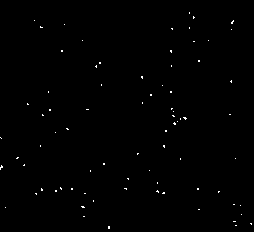
\includegraphics[width=8.5cm]{./images/bacteriasmall_threshold}
        \caption{This represents a segmented and inverted version of the image on the left. White cluster are bacteria.}\label{BBB}
    \end{minipage}
\end{figure*}
In this section we present an application of TraCCA to the analysis of motion of \textit{B. subtilis.}
The analysis of trajectories in bacteria is really interesting because it is a non-invasive way of extracting much information about their chemotaxis which is the ability of bacteria to sense and respond to chemicals.
Thanks to chemotaxis, bacteria are able to reach a source of nutrient and move away from repellents, which makes it a key characteristic for their survival. Studying chemotaxis is really interesting not only because it has a strong influence on many biological mechanisms, e.g. biofilm formation and disease pathogenesis but also because  evolution's natural selection has optimized bacterial chemotaxis making bacteria excellent source-seekers and their strategies can be used to design bio-inspired, simple and efficient algorithms for robotic source locating systems. 
The motility  of \textit{B. subtilis} is composed of a series of \textit{run} (bacteria swim along smooth segments) and \textit{``tumbles''} (cells stop and randomly select a new direction).
Combining run and tumbles bacteria are able to direct their motility in order to reach nutrients and move away from repellent, in other words, to do their chemotaxis.
An algorithm that is able to track bacteria is really useful  because from bacterial trajectories much information about the way bacteria perform chemotaxis (e.g. duration of the run, swimming speed, frequency of tumbling events) can be extracted. 
This information is important in studying the strategy they adopt to reach a source of nutrient; moreover it is also interesting to investigating how the trajectories changes as certain environmental conditions change, such as temperature, oxygen concentration or gradient of chemicals.


In this work we used \textit{B. subtilis} strain \texttt{OI1085} for the tracking experiment.
Cells were taken from frozen stock, resuspended in CAM (Cap Assay Minimal) and shaken  (\SI{37}{\degree}, 100 rpm) until the optical density $OD600=0.3$ was reached; we then diluted the suspension 1:10 in CAM.
The bacterial suspension was injected in a micro-fluidic device.
The micro-fluidic device is a simple device made by \textit{PDMS} and glass, composed of three parallel channels (height 100 um).
In the central channel ( \SI{600}{\micro\meter} wide) bacteria were hosted and observed.
Two  walls of \textit{PDMS} (\SI{200}{\micro\metre}) separate the central channel from the left and right channels were oxygen was flown in order to reach a concentration of oxygen closed to 100\% in the central channel.
10 minutes after the injection of bacterial suspension a video was acquired at 100 frames per second for \SI{41}{\second}  (\#4100 frames). All images were acquired through a 10$\times$ phase contrast objective (\textit{Nikon} microscope), using binning $2 \times 2$.
All images are $512 \times 512$ pixels and have been exported in $16$-bit grayscale \texttt{TIFF} image format.




\subsection{Bacteria Segmentation}

The \textit{B. subtilis} cells typically have a large range of motion patterns and the cell soma generally appears as a dark area surrounded with a white halo.
Colors can be inverted and the cell may appear white when it  moves out of focus sufficiently (see Figure \ref{contrast}).
In order to automatically detect \textit{subtilis} cells in each frame, it is possible to use a histogram-based thresholding method as suggested in \cite{Cho:1989}.
A key step of tracking bacteria is to individuate first, and then to label and describe each of the bacteria present in the images.
In order to do so a segmentation preprocessing phase is performed on all the images. 
Segmentation  is carried out by means of a threshold method \cite{Shapiro:2002} which produces a bi-partition of the pixel based on the color intensity. The value of pixel $(x,y)$ in image $g$ is given by the following, where $P$ is a predicate and f is the original image:
${g(x,y) = \begin{cases} 1, & \mbox{if } P(f(x,y),T) \\ 0, & \mbox{otherwise }\end{cases}}$.
One drawback of using threshold method is that pixel color intensity is the only property being considerend by the bi-partition process, not any relationships between the pixels. This can easily lead to binary regions where pixels are not contiguous or to miss or include relevant or unwanted pixels respectively.
These effects can get worse as the noise increases. For the problem at hand, however, the threshold method works well because after the application of a \texttt{contrast stretch filter} the analysed images presents high contrasts between the background and cells soma (see figure \ref{contrast}).
Contrast stretch filter  stretches or scales the range of pixel values between an upper and lower limit.
Pixel values that are above or below this range are saturated to the upper or lower limit values respectively, while pixels that lies in the interval are scaled according to the following formula: 
\[{g(x,y) = \begin{cases} L_o & \mbox{if } f(x,y) < L_i \\  H_o & \mbox{if } f(x,y) < H_i\\ L_o + (f(x,y)-L_i)\frac{H_o-L_o}{H_i-L_i} & \mbox{if } L_i \leq f(x,y) \leq H_i\end{cases}}\] where  $[L_i,H_i]$ defines the interval in the original image which is linearly scaled into the interval $[L_o,H_o]$.

All the images go through a noise reduction stage which employs a combinations of \textit{gaussian}, \textit{laplacian} and \textit{blurring} filters \cite{Deng:1993}.
Values parameters used in the Contrast Stretching and Threshold filters are dataset dependent and need to be provided upfront. The initial range of colors is affected by optical conditions at the time of the experiment such as lenses, luminosity etc.
Once the best set of parameters for one image are found, they can be used throughout the whole dataset since all images are taken under the same conditions.


\subsection{Bacteria Tracking}

Binary images are then used to extract the relevant information for each of the segmented bacteria. This is done by interpreting each image as a graph whose nodes are pixels and an arc $(i,j)$ exists if pixels $i$ and $j$ are set and neighbors (according to \textit{Moore}'s relationship, see section \ref{sec:CA}).
Bacteria correspond then to a connected component that are easily individuated by using an elementary processes which triggers a DFS visit from each set pixel. Once all pixels that make up the cell soma are individuated a unique ID $id_i$ that  identifies the bacterium uniquely, a centroid $c_i$ and a bounding box $s_i$ which describe describes the location, the shape and the area respectively are computed for each bacterium $i$. \texttt{CGAL} \cite{CGAL} is used to create and manipulate any geometrical entities. All the bacteria whose extension is less than $M_e = 2$\textit{px} are ignored and no further considered.

Weight function is a linear combination of the centroids distance and shapes difference 
\begin{equation}
\label{sec:bacttracking}
W(c_i,c_j) = a \sqrt{(x_{c_i} - x_{c_j})^2 + (y_{c_i}-y_{c_j})^2} + b |S_i \cap S_j|
\end{equation}
where $S_i$ and $S_j$ are the sets of pixels within the boundaries of the bacteria's  bounding box.






\section{Analysis and Validation}
Starting from the relationship $D_b=  \frac{v^2 t_t}{2}$  \cite{Berg:1993} that links the diffusion coefficient to both swim velocity ($v$) and tumbling time ($tt$), 
we have separated each trajectory into running and tumbling events \footnote{An additional validation has been performed, which, for the sake of brevity is only outlined here, uses \textit{Mean Square Displacement} (\texttt{MSD}) in time and considering the following relationship $MSD(t)=\frac{1}{2}\frac{v^2 t_R^2}{2t/t_R +e^{\frac{-2t}{t_R}-1}}$ \cite{Howse:2007} where $v$ is the swimming speed, $t_R$ is the timescale associated to rotational diffusion that is $t_R=2t_t$, it is possible to obtain $t_R $ and $v$ via fitting. $t_t$ and $v$ are then used to compute $D_b$}. 

Those events allow the swimming speed to be calculated as difference between subsequent bacteria positions.
The tumbling time can be calculated as the time spent tumbling divided by the number of tumbling events. 
Inspired by the work of \textit{Wong-Ng et al.} \cite{Wong2016} and \textit{B. Masson et al.} \cite{Masson:2011} we wrote an algorithm, implemented in \textit{MATLAB}, which detects such running/tumbling events (see Figure \ref{runtumbledetection}) which in turn were used to extract all the relevant biological information about bacteria motion from the tracked trajectories\footnote{Tumbles are associated to a decrease in advancing velocity and an abrupt change in the angular velocity (i.e. in the direction of the motion). Fixing a threshold on both advancing and angular velocities it is possible to identify running/tumbling and use them to computes the mean values $t_t$ and $v$ over all the trajectories of the experiment.}.
    \begin{figure}[htp]
         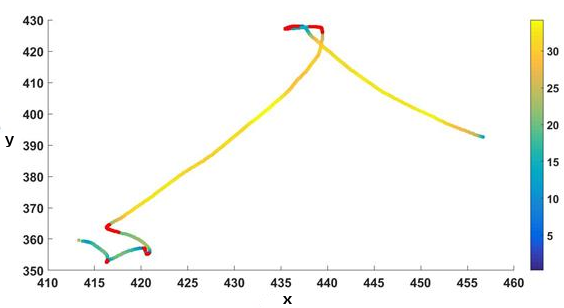
\includegraphics[width=9.3cm,height=7cm]{./images/runtumble.png}
        \caption{This figure depicts the tracked trajectory of a single bacterium. Blue-yellow colors gradient shows the velocity. The red segments represent the identifies tumbles.}
        \label{runtumbledetection}
    \end{figure}

We found a mean swimming velocity of  \SI{18}{\micro\meter \per \second}, a mean run time (time spent swimming straight) of \SI{0.8}{\second} and a tumble time of \SI{0.18}{\second}. 
All these values are in accordance with the results of \textit{Cisneros et al.} \cite{Cisneros:2011}.

\section{Conclusion}\label{conclusions}
This premiliary work we presented a an cellular automata based framework for tracking centroid-bounding box represented particles. 
We also presented an application of the proposed framework on tracking the motion of \textit{B. subtilis} in a microfliudic device in order to retrieve the average swimming velocity, running and tumble times. The results are in accordance with \cite{Cisneros:2011}. 
\subsection{Future works}
Due to the possible large number of particles and frames involved in such analysis a parallel GPGPU+MPI version of the framework is being developed and it will be applied to the analisys of a much larger dataset to test its scalability and speedup.
It is also important to note that under the assumption of associativity of the \textit{assignment operator} $\lozenge$ the tracking algorithm could be implemented using the design pattern of \textit{parallel reduction}.

    \begin{figure}[h]
      \begin{center}
        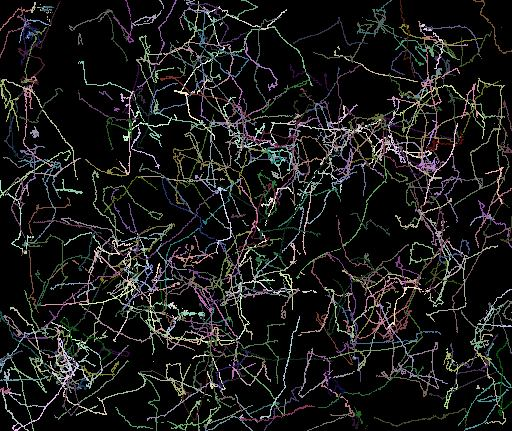
\includegraphics[scale=0.5]{./images/result.png}
        \caption{This figures shows the collective view of all the tracked bacteria tracjectories. A random color is associated to each trajectory.}\label{fig:}
        
      \end{center}
    \end{figure}


% if have a single appendix:
%\appendix[Proof of the Zonklar Equations]
% or
%\appendix  % for no appendix heading
% do not use \section anymore after \appendix, only \section*
% is possibly needed

% use appendices with more than one appendix
% then use \section to start each appendix
% you must declare a \section before using any
% \subsection or using \label (\appendices by itself
% starts a section numbered zero.)
%


%\appendices
%\section{Images Filters}
%\subsection{Contrast stretch}

% use section* for acknowledgement
\section*{Acknowledgment}
The authors would like to thank NVIDIA for providing GPUs and Prof. Filippo Melascina from the University of Edinburgh, Institute of BioEngineering, UK who kindly gave access to the microscopy equipment.


% Can use something like this to put references on a page
% by themselves when using endfloat and the captionsoff option.
\ifCLASSOPTIONcaptionsoff
  \newpage
\fi



% trigger a \newpage just before the given reference
% number - used to balance the columns on the last page
% adjust value as needed - may need to be readjusted if
% the document is modified later
%\IEEEtriggeratref{8}
% The "triggered" command can be changed if desired:
 ì%\IEEEtriggercmd{\enlargethispage{-5in}}

% references section

% can use a bibliography generated by BibTeX as a .bbl file
% BibTeX documentation can be easily obtained at:
% http://www.ctan.org/tex-archive/biblio/bibtex/contrib/doc/
% The IEEEtran BibTeX style support page is at:
% http://www.michaelshell.org/tex/ieeetran/bibtex/
%\bibliographystyle{IEEEtran}
% argument is your BibTeX string definitions and bibliography database(s)
%\bibliography{IEEEabrv,../bib/paper}
%
% <OR> manually copy in the resultant .bbl file
% set second argument of \begin to the number of references
% (used to reserve space for the reference number labels box)
\begin{thebibliography}{1}

\bibitem{Cho:1989}
S. Cho, R. Haralick, and S. Yi, ``Improvement of Kittler and Illingworth’s minimum error thresholding,'' Pattern Recognit., vol. 22, no. 5, pp. 609– 617, 1989.
\bibitem{Shapiro:2002}
Shapiro, Linda G, Stockman, George C. (2002). "Computer Vision". Prentice Hall. ISBN 0-13-030796-3

\bibitem{Deng:1993} 
G. Deng and L. W. Cahill, An adaptive Gaussian filter for noise reduction and edge detection, Nuclear Science Symposium and Medical Imaging Conference, 1993. 1615-1619 vol.3, 10.1109/NSSMIC.1993.373563

\bibitem{CGAL}
CGAL, Computational Geometry Algorithms Library, http://www.cgal.org
\bibitem{bellmann1978}
Bellman, R. E. Review: Eugene L. Lawler, Combinatorial optimization: networks and matroids . 
 Bull. Amer. Math. Soc. 84 (1978)



\bibitem{opencalurl}
OPENCAL download page: \url{https://github.com/OpenCALTeam/opencal/releases}
\bibitem{opencalmanual}
OPENCAL download page: \url{https://github.com/OpenCALTeam/opencal-user-guide}

\bibitem{msdanalyzer}
Nadine Tarantino, Jean-Yves Tinevez, Elizabeth Faris Crowell, Bertrand Boisson, Ricardo Henriques, Musa Mhlanga, Fabrice Agou, Alain Israël, and Emmanuel Laplantine. TNF and IL-1 exhibit distinct ubiquitin requirements for inducing NEMO-IKK supramolecular structures. J Cell Biol (2014) vol. 204 (2) pp. 231-45

\bibitem{msdanalyzer:web}
\url{http://tinevez.github.io/msdanalyzer/}

\bibitem{Wong2016}
Wong-Ng J, Melbinger A, Celani A, Vergassola M (2016) The Role of Adaptation in Bacterial Speed Races. PLoS Comput Biol 12(6): e1004974. doi: 10.1371/journal.pcbi.1004974

\bibitem{Masson:2011}
Noninvasive inference of the molecular chemotactic response using bacterial trajectories Jean-Baptiste Masson, Guillaume Voisinnea, Jerome Wong-Nga, Antonio Celania, and Massimo Vergassola, 2011

\bibitem{Cisneros:2011}
Cisneros, L. H., Kessler, J. O., Ganguly, S.,  Goldstein, R. E. (2011). Dynamics of swimming bacteria: Transition to directional order at high concentration. Physical Review E, 83(6), 061907.

\bibitem{toti1999}
Salvatore Di Gregorio, Roberto Serra, An empirical method for modelling and simulating some complex macroscopic phenomena by cellular automata, Future Generation Computer Systems, Volume 16, Issues 2–3, December 1999, pp. 259-271.

\bibitem{spataro2014}
Spataro, Davide, et al. "The new SCIARA-fv3 numerical model and acceleration by GPGPU strategies." International Journal of High Performance Computing Applications (2015)


\bibitem{Neumann1966}
John Von Neumann. 1966. Theory of Self-Reproducing Automata. Arthur W. Burks (Ed.). University of Illinois Press, Champaign, IL, USA

\end{thebibliography}

% biography section
% 
% If you have an EPS/PDF photo (graphicx package needed) extra braces are
% needed around the contents of the optional argument to biography to prevent
% the LaTeX parser from getting confused when it sees the complicated
% \includegraphics command within an optional argument. (You could create
% your own custom macro containing the \includegraphics command to make things
% simpler here.)
%\begin{biography}[{\includegraphics[width=1in,height=1.25in,clip,keepaspectratio]{mshell}}]{Michael Shell}
% or if you just want to reserve a space for a photo:

\begin{IEEEbiography}[{\includegraphics[width=1in,height=1.25in,clip,keepaspectratio]{picture}}]{John Doe}
\blindtext
\end{IEEEbiography}

% You can push biographies down or up by placing
% a \vfill before or after them. The appropriate
% use of \vfill depends on what kind of text is
% on the last page and whether or not the columns
% are being equalized.

%\vfill

% Can be used to pull up biographies so that the bottom of the last one
% is flush with the other column.
%\enlargethispage{-5in}

\end{document}


